\chapter{Appendix}

\section{Testfälle} \label{tests}

\begin{longtable}{|p{1cm} | p{10cm} |p{1.2cm}|}
  \hline
    ID & Ablauf & Erfüllt \\\hline
    T1 & \gls{ikc-core} starten ohne das ein Index existiert. Anschliessend müssen alle Daten eingelesen werden, der Index generiert und gespeichert werden& \\\hline
    T2 & \gls{ikc-core} starten während eine Index existiert jedoch nicht eingelesen ist. Nun muss der Indexgeladen werden und allfällige Änderungen (neue oder geänderte Dateien) nach getragen werden.&\\\hline
    T3 & \gls{ikc-core} starten und der Index ist aktuell und initialisiert. In diesem Fall muss nach kurzer Zeit die Rückmeldung kommen, dass der Index bereit ist.&\\\hline
    T4 & Innerhalb der Suche, müssen neben lokalen Suchresultate auch solche aus dem Volltext Index erscheinen. &\\\hline
    T5 & Sobald ein externes Dokument geladen wird, müssen die \gls{Keyphrase}[s] abgefragt und dargestellt werden.&\\\hline
    T6 & Wird ein \gls{Keyphrase} ausgewählt müssen alle dazugehörigen Dokumente abgefragt und angezeigt werden.&\\\hline
    T7 & Wenn ein neues Text Dokument innerhalb der externen Datenquelle erstellt wurde muss dieses beim nächsten Abgleich mit dem generierten Index verarbeitet werden.&\\\hline
    T8 & Wenn ein neues Text Dokument innerhalb der externen Datenquelle geändert wurde muss dieses beim nächsten Abgleich mit dem generierten Index verarbeitet werden.&\\\hline
    \caption{Testfälle Beschreibung}
  \label{tab:testkonzept-detail}
\end{longtable}



\section{Arbeitsjournal}
\label{arbeitsjournal}

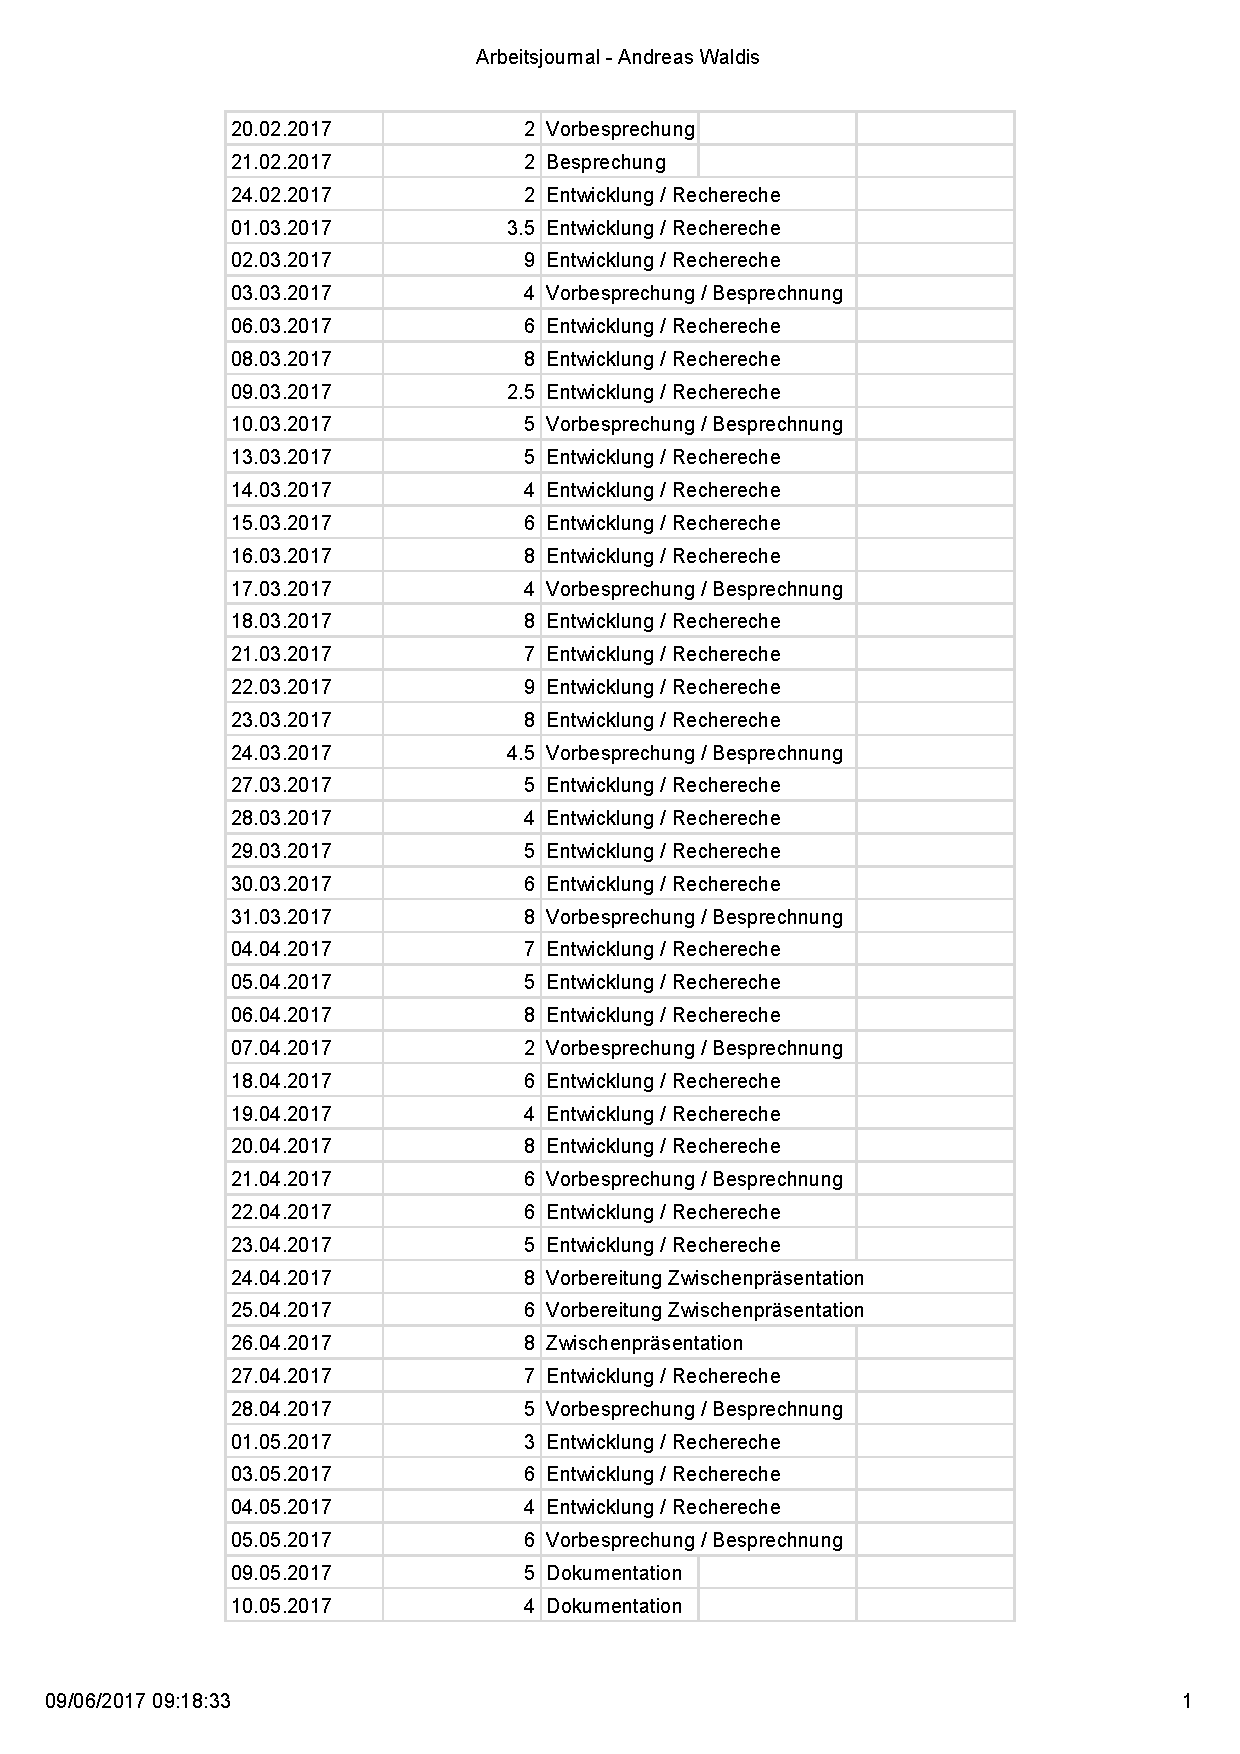
\includegraphics[page=1,scale=0.8]{bilder/Arbeitsjournal.pdf}
\includegraphics[page=2,scale=0.8]{bilder/Arbeitsjournal.pdf}
\includegraphics[page=3,scale=0.8]{bilder/Arbeitsjournal.pdf}
\includegraphics[page=4,scale=0.8]{bilder/Arbeitsjournal.pdf}

\section{Aufgabenstellung}
\label{aufgabenstellung}


\includegraphics[page=1,scale=0.8]{bilder/Aufgabenstellung.pdf}

\includegraphics[page=2,scale=0.8]{bilder/Aufgabenstellung.pdf}

\includegraphics[page=3,scale=0.8]{bilder/Aufgabenstellung.pdf}

\includegraphics[page=4,scale=0.8]{bilder/Aufgabenstellung.pdf}


\section{Anforderungsanalyse}\label{anforderungsanalyse-mk}

\includegraphics[page=1,scale=0.8]{kapitel/anforderungen.pdf}

\includegraphics[page=2,scale=0.8]{kapitel/anforderungen.pdf}

\includegraphics[page=3,scale=0.8]{kapitel/anforderungen.pdf}

\includegraphics[page=4,scale=0.8]{kapitel/anforderungen.pdf}

\section{Projektmanagement}

\newpage

\subsection{Projektstrukturplan}
\begin{landscape}
\begin{figure}[ht]
\centering
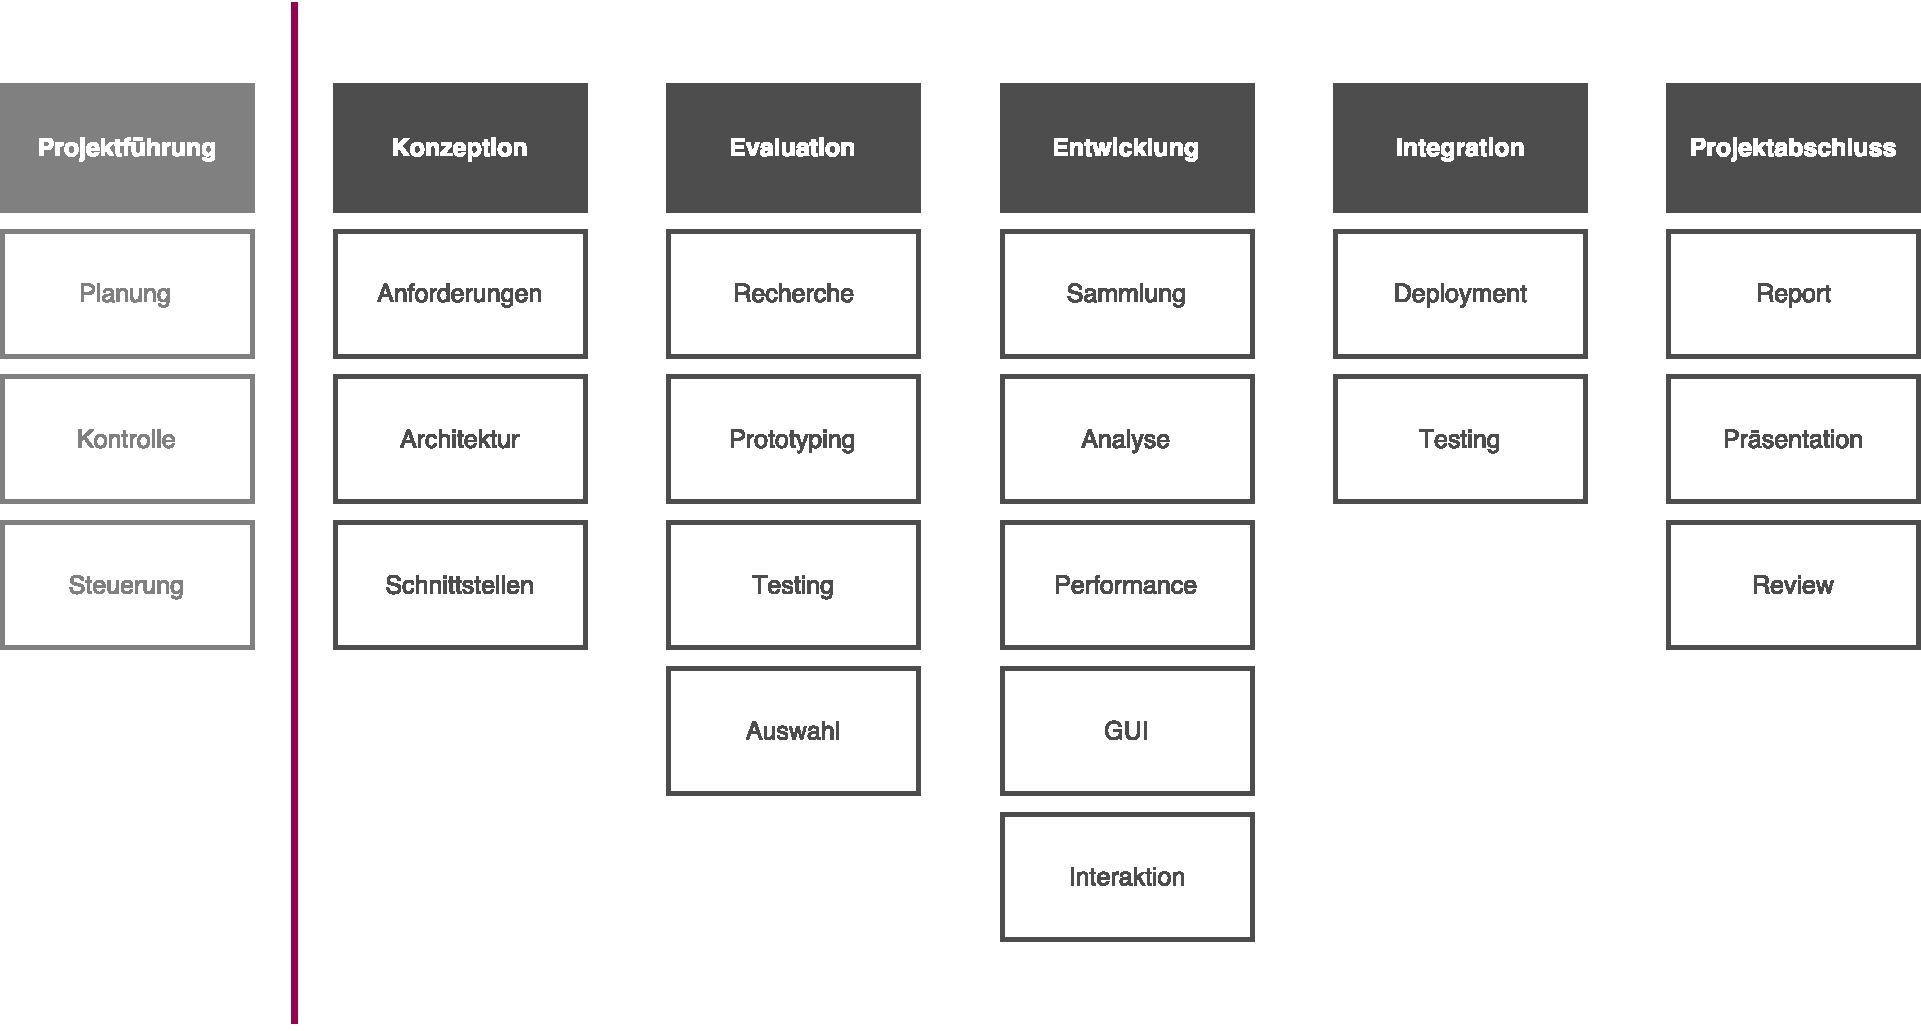
\includegraphics[width=1.5\textwidth]{Projektstrukturplan}
\caption{Projektstrukturplan}
\label{fig:projektstrukturplan}
\end{figure}
\end{landscape}

\newpage
\subsection{Meilensteine}

\begin{longtable}{|p{1cm}|p{2cm}|p{8.5cm}|}
  \hline
    ID & Kalenderwoche &  Beschreibung \\\hline
    M1 & KW11 & Projektsetup erstellt\\\hline
    M2 & KW13 & Sprint 2 abgeschlossen\\\hline
    M3 & KW15 & Sprint 3 abgeschlossen\\\hline
    M4 & KW17 & Sprint 4 abgeschlossen\\\hline
    M5 & KW19-20 & Sprint 5 abgeschlossen\\\hline
    M6 & KW22 & Sprint 6 abgeschlossen\\\hline
    M1' & KW17-18 & Zwischenpräsentation\\\hline
    M2' & KW25-26 & Abschlusspräsentation\\\hline
    \caption{Meilensteine}
  \label{tab:meilensteine}
\end{longtable}
\subsection{Rahmenplanung}
\newpage

\begin{landscape}
\begin{figure}[ht]
\centering
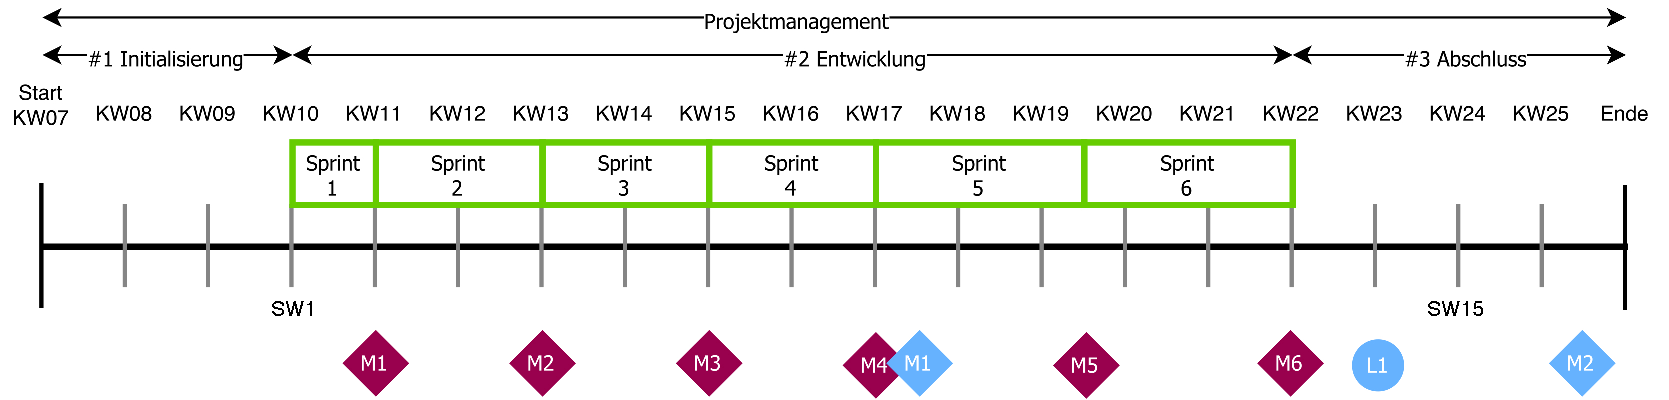
\includegraphics[width=1.7\textwidth]{Rahmenplan-sw}
\caption{Rahmenplan}
\label{fig:rahmenplan}
\end{figure}
\end{landscape}

\newpage

\subsection{Anforderungen}\label{anforderungen}
\begin{longtable}{|p{1.5cm} | p{1.5cm} | p{8.1cm}|}
  \hline
    ID & Priorität & Beschreibung \\\hline
    A1 & M & \gls{Datenquelle}[n] können mittels einer Autoindexierung automatisch in die Volltextsuche inventarisiert werden.\\\hline
    A2 & S & Neue oder geänderte Dateien können im bestehenden Index hinzugefügt oder geändert werden (z.B. automatisch nach Änderungs- oder Erstellungsdatum). Es ist zu prüfen, wie diese Änderung sich auf die bestehenden Tags auswirkt. \\\hline
    A3 & S  & Die zu indexierenden \gls{Datenquelle}[n] können vom Benutzer ausgewählt werden.\\\hline
    A4 & M & Mittels der Volltextsuche sollen sowohl alle Knoten, als auch alle in den \gls{Datenquelle}[n] enthaltenen Dokumente, welche in der Autoindexierung erfasst sind, durchsucht werden können.\\\hline
    A5 & M & Die Volltextsuche kann über ein Suchfeld genutzt werden.\\\hline
    A6 & C & Dabei sollen die unterschiedlichen Quellen der Resultate visuell unterschieden werden können.\\\hline
    A7 & M & Basierend auf dem Inhalt des Wissensnetzwerks sollen \gls{Keyword}[s] berechnet und dem User zur Verknüpfung vorgeschlagen werden.\\\hline
    A8 & M & Die automatisch generierten \gls{Keyword}[s] sind klar als solche gekennzeichnet und können vom Benutzer angenommen oder abgelehnt werden. (\gls{Tag Recommondation})\\\hline
    A9 & C & Mittels \gls{Tags} kann der Benutzer weitere Informationen zu Knoten hinzufügen.\\\hline
    A10 & C & Bestehende \gls{Tag}[s] sollen dem Benutzer vorgeschlagen werden.\\\hline
    A11 & M & Jedes Dokument, das der Benutzer in sein Netzwerk hinzufügt, wird als ein Knoten im Wissensnetzwerk eingefügt. Jeder \gls{Tag} eines solchen Dokuments wird auch als Knoten im Wissensnetzwerk eingefügt. Die zugehörigen Tags werden als  Links zwischen den Tag-Knoten und den Dokument-Knoten verbunden.\\\hline
    A12 & M & \gls{Tag}[s] werden dem User differenziert von den anderen Eigenschaften dargestellt.\\\hline
    A13 & C & Zusammengesetze Wörter (\gls{N-Gramm}[e]) werden als solche erkannt und entsprechend in der \gls{Keyword Extraction} berücksichtigt. \\\hline
    A14 & S & \gls{SFTP} Persistenz (DB), Index, Konfiguration \\\hline
    A15 & C & \gls{Dropbox} Persistenz (DB), Index, Konfiguration \\\hline
    A16 & C & \gls{Evernote} Index, Konfiguration \\\hline
    %A1 & M & Implementation einer Funktion \texttt{getRelevantTerms(Doc)}, welche pro Dokument eine sortierte Liste (nach tf-idf-Relevanz) von \gls{Keyword}[s] zurückgibt.\\\hline
    \caption{Funktionale Anforderungen}
  \label{tab:funktionale-anforderungen}
\end{longtable}

\begin{longtable}{|p{1.5cm} | p{1.5cm} | p{8.1cm}|}
  \hline
    ID & Priorität & Beschreibung \\\hline
    A1 & M & Die Autoindexierung soll den Benutzer nicht in der Bedienung blockieren (Usability).\\\hline
    A2 & M & Die \gls{Keyword Extraction} ist innerhalb nützlicher Frist abzulaufen. \\\hline
    A3 & S & Generische Einbindung der Quelle (zum Beispiel Factory-Pattern) für eine einfache Anbindung neuer Quellen.\\\hline
    A4 & M  & 360 Stunden pro Person\\\hline
    A5 & S & Arbeitsjournal \\\hline
    A6 & S & Weiterentwicklung des \gls{ikc-core}[s] \\\hline
    \caption{Nicht funktionale Anforderungen}
  \label{tab:nicht-funktionale-anforderungen}
\end{longtable}

\subsection{Risikoanalyse}\label{risikoanalyse}

In folgender \autoref{tab:risikoanalyse} werden mögliche Risiken behandelt. Die Wahrscheinlichkeit ist mit P abgekürzt. R steht für Risiko und S für den Schaden, welcher mittels $P*R=S$ berechnet wird. Die Skala reicht von eins bis fünf.

\clearpage

\begin{longtable}{|p{0.5cm} | p{7cm} | p{1cm}|  p{1cm}|  p{1cm}|}
  \hline
    ID & Beschreibung &  P & R & S \\\hline
    R1 & Die für eine reibungslose und intuitive Bedienung nötige Performance kann nicht gewährleistet werden.\newline\newline
    Javascript ist sowohl auf dem Client als auch auf dem Server lauffähig. Damit kann jeweils auf die für den Anwendungsfall nötige Plattform gewechselt werden. & 3 & 4 & 12\\\hline
    R2 & Die Abgrenzung vom laufenden Projekt \textbf{\acrshort{IKC}} (vgl. \autoref{sec:scope}) ist klar festzulegen und einzuhalten. So können Überschneidungen und Unklarheiten verhindert werden.\newline\newline
    Vollständige und detaillierte Arbeitsjournale, wie auch Protokolle bieten dabei eine wichtige Hilfestellung. & 2 & 1 & 2\\\hline
    R3 & Die Zahl und auch der Schwierigkeitsgrad der Anforderungen ist hoch. Die Arbeit ist mit insgesamt 720 Stunden in einem grösseren Rahmen. Es ist daher möglich, dass nicht alle Anforderungen erfüllt werden.\newline\newline Eine strikte Priorisierung und ein funktionierendes Projektmanagement garantiert, dass wichtige Anforderungen erkannt und gleichzeitig auch nicht aus den Augen verloren werden. & 3 & 1 & 3\\\hline
    R4 & Typescript (beziehungsweise Javascript) ist für den Einsatzzweck nicht vollends geeignet und schränkt die Performance und oder den Einsatz von bestimmten Bibliotheken ein.\newline\newline
    Das Resultat dieser Arbeit ist ein Prototyp. Das Ziel ist damit den Mehrwert aus dem zusätzlichen Wissen aufzuzeigen. Sollte die Performance mit den genutzten Technologien nicht ausreichend sein, können dennoch diverse Konzepte und Erkenntnisse in einem Folgeprojekt wiederverwendet und weiterentwickelt werden.& 3 & 3 & 9\\\hline
    R5 & Demo-Daten und nur englische Dokumente & 3 & 1 & 3\\\hline
    \caption{Risikoanalyse}
  \label{tab:risikoanalyse}
\end{longtable}

\subsection{Lieferobjekte}\label{lieferobjekte}

\begin{longtable}{|p{1cm} | p{2cm} | p{8.1cm}|}
  \hline
    ID & Datum &  Beschreibung \\\hline
    L1 & 26.04.2017 & Zwischenpräsentation.\\\hline
    L2 & 09.06.2017 & Funktionsfähige Software gemäss den Anforderungen
    \\\hline
    L3 & 09.06.2017 & Dokumentierter Sourcecode (für Methoden und Parameter).\\\hline
    L4 & 09.06.2017 & \gls{BDA}-Bericht.\\\hline
    \caption{Vorgegebene Lieferobjekte}
  \label{tab:set-lieferobjekte}
\end{longtable}
 
\begin{longtable}{|p{1cm} | p{2cm} | p{8.1cm}|}
  \hline
    ID & Datum &  Beschreibung \\\hline
    L1' & 24.03.2017 & Abschluss der Anforderungsanalyse.\\\hline
    L2' & 31.03.2017 & Konzeptioneller Prototyp, welcher aufgrund der Resultate der Technologierecherche entwickelt wurde.\\\hline
    L3' & 14.04.2017 & Integration des Prototypen in den \gls{ikc-core}\\\hline
    L3' & 26.05.2017 & Abschluss der Programmierung.\\\hline
    \caption{Zusätzliche, interne Lieferobjekte}
  \label{tab:add-lieferobjekte}
\end{longtable}



\subsection{Stories}
Die User-Stories repräsentieren alle Arbeitspakete, welche über die gesamte Projektdauer geplant wurden. Diese werden nicht nur im klassischen Sinne für die Klassifizierung von Applikationsfunktionen, sondern auch für konzeptionelle Aufgaben verwendet. Insgesamt wurde der Aufwand mit \textbf{560} Punkte beziffert, wobei ein Punkt circa einer Stunde entspricht. Dies entspricht auch etwa dem resultierenden Aufwand von \textbf{580} Punkten. Der Mehraufwand konnte dank einiger Reserven gut kompensiert werden. Dieser entstand vor allem in der Umsetzung der \gls{Drag'n'Drop} Gesten und dem Datenaustausch zwischen \gls{ikc-core} und Visualisierung. Alle User-Stories sind in der \autoref{user-stories} detailliert aufgelistet.

\begin{longtable}{|p{0.6cm}|P{4.5cm}|p{1.4cm}|p{1.4cm}|p{2.4cm}|}
\hline
ID  & Name & Geplant & Effektiv &Sprint\\ \hline
S1 & Technologierecherche           & 70 pt             &  80pt              & 1, 2 \\ \hline
S2 & Definition Projektrahmen           & 20 pt             &  10pt              & 1  \\ \hline
S3 & Entwurf Anforderungen           & 20 pt             &  10pt              & 1 \\ \hline
S4 & Setup Dokumentation           & 20 pt             &  25pt              & 1 \\ \hline
S5 & Prototype Keyword Extraktion            & 80 pt             &  75pt              & 2 \\ \hline
S6 & Tokenauthentifizierung           & 35 pt             &  50pt              & 2 \\ \hline
S7 & Keyword Extraktion grosser Index          & 45 pt             &  50pt              & 2, 3 \\ \hline
S8 & Integration Suche in Index in Benutzeroberfläche           & 20 pt             &  20pt             & 3 \\ \hline
S9 & Keyword Extraktion für bestimmtes Dokument         & 20 pt             &  15pt              & 3 \\ \hline
S10 & Extraktion aller Dokumente für ein Keyword       & 20 pt             &  20pt              & 3 \\ \hline
S11 & Optimierung Keyword Extraktion Algorithmus    & 150 pt             &  160pt              & 3,4,6 \\ \hline
S12 & Begrenzung der extrahierten Keywords    & 60 pt             &  50pt              & 3,4,6 \\ \hline
S13 & Begrenzung Dokumente für Keywords    & 20 pt             &  15pt              & 3,4,6 \\ \hline
\hline
 & \textbf{Total}                       & \textbf{560 pt}& \textbf{580 pt}&   \\\hline
    \caption{User Stories}
 \label{user-stories}
\end{longtable}

\subsection{Testkonzept}
Basierend auf den \hyperref[anforderungen]{Anforderungen} wurden die verschiedenen Testfälle definiert. Diese sind hier zusammengefasst. Konkret handelt es sich um die folgenden Testfälle (\autoref{tab:testkonzept}), welche im \autoref{tests} genauer beschrieben sind.

\begin{longtable}{|p{1cm} | P{6cm} |}
  \hline
    ID & Kurzbeschrieb \\\hline
    T1 & \gls{ikc-core} starten, Index existiert nicht.\\\hline
    T2 & \gls{ikc-core} starten, Index existiert ist jedoch nicht initialisiert.\\\hline
    T3 & \gls{ikc-core} starten, Index existiert und ist initialisiert.\\\hline
    T4 & Dokument suchen innerhalb des Index.\\\hline
    T5 & \gls{Keyword}[s] für ein Dokument abfragen.\\\hline
    T6 & Dokumente für \gls{Keyword} abfragen.\\\hline
    T7 & Neues Dokument erstellen.\\\hline
    T8 & Dokument ändern.\\\hline
    \caption{Testfälle}
  \label{tab:testkonzept}
\end{longtable}

\section{Benutzerhandbuch}\label{tutorial}

\subsection{Konfiguration}

Mit Hilfe der Konfiguration können verschiedenen Aspekte des \gls{ikc-core}[s] als auch des Prototypen angepasst werden. Sie ist aufgeteilt in drei Bereiche:
\begin{enumerate}
    \item Die \textbf{MetaDataConfig} (\autoref{fig:meta-config}) enthält die Verbindungsinformationen für die Speicherung der Metadaten des \gls{ikc-core}[s]:
    \begin{itemize}
        \item \textbf{SFTP Url}: die Adresse des \gls{SFTP} Servers.
        \item \textbf{Path}, der Pfad zu den Metadaten auf dem \gls{SFTP}-Server.
        \item \textbf{User}: der Benutzer für die Verbindung.
        \item \textbf{SSH-Key}: der Schlüssel, um sich auf den \gls{SFTP}-Server zu verbinden. 
    \end{itemize}
    \item Die \textbf{GlobalConfig} (\autoref{fig:global-config}) enthält die folgenden globalen Parameter:
    \begin{itemize}
        \item \textbf{Index Service Url}: die Url für die Verbindung zum \textit{IndexService} (via \textit{HTTPS} oder \textit{WSS}).
        \item \textbf{Data Service Url}: die Url für die Verbindung zum \textit{DataService} (ebenfalls via \textit{HTTPS} oder \textit{WSS}).
        \item \textbf{Extraction Threshold}: definiert den Schwellenwert für die Extraktion von \gls{Keyphrase}[s].
        \item \textbf{Minimum Documents}: definiert, in wie vielen Dokumenten eine relevante \gls{Keyphrase} mindestens vorkommen muss.
    \end{itemize}
    \item \textbf{SFTPConfig} (\autoref{fig:sftp-config}): enthält die Verbindungsinformationen, um auf den \gls{SFTP}-Server zuzugreifen und die externen Daten einzulesen. Dabei müssen die gleichen Parameter, wie in \textbf{MetaDataConfig}, definiert werden.
\end{enumerate}

\newpage
\begin{landscape}

\begin{figure}[htbp]
    \centering
    \begin{subfigure}[b]{0.5\textwidth}
    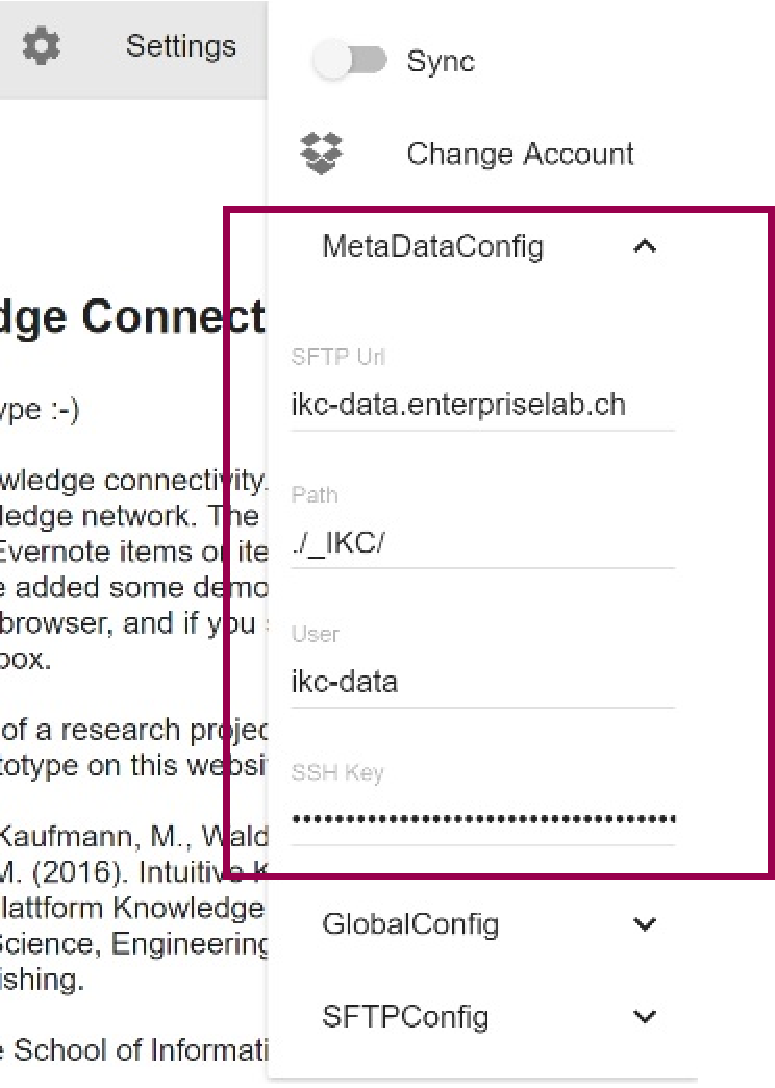
\includegraphics[width=1\linewidth]{Settings-Meta}
    \caption{MetaData}
    \label{fig:meta-config}
    \end{subfigure}
     \begin{subfigure}[b]{0.3\textwidth}
    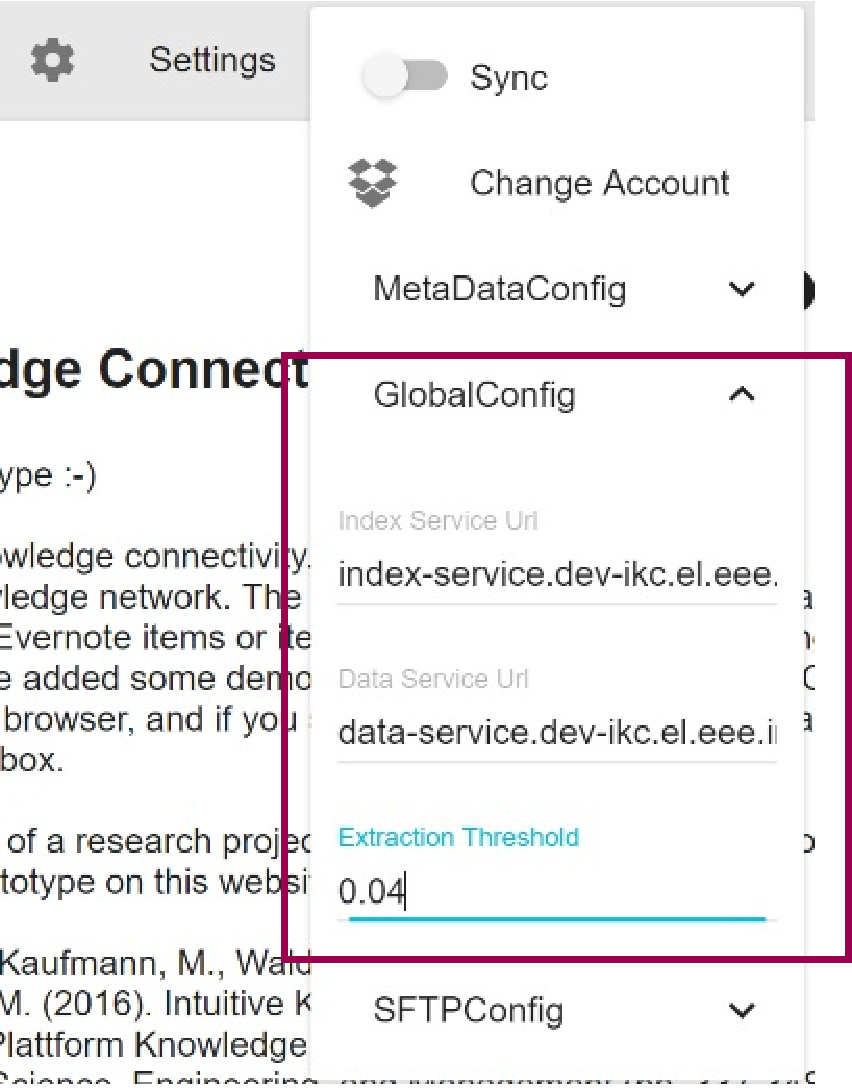
\includegraphics[width=1\linewidth]{Settings-Global}
    \caption{Globale}
    \label{fig:global-config}
    \end{subfigure}
     \begin{subfigure}[b]{0.5\textwidth}
    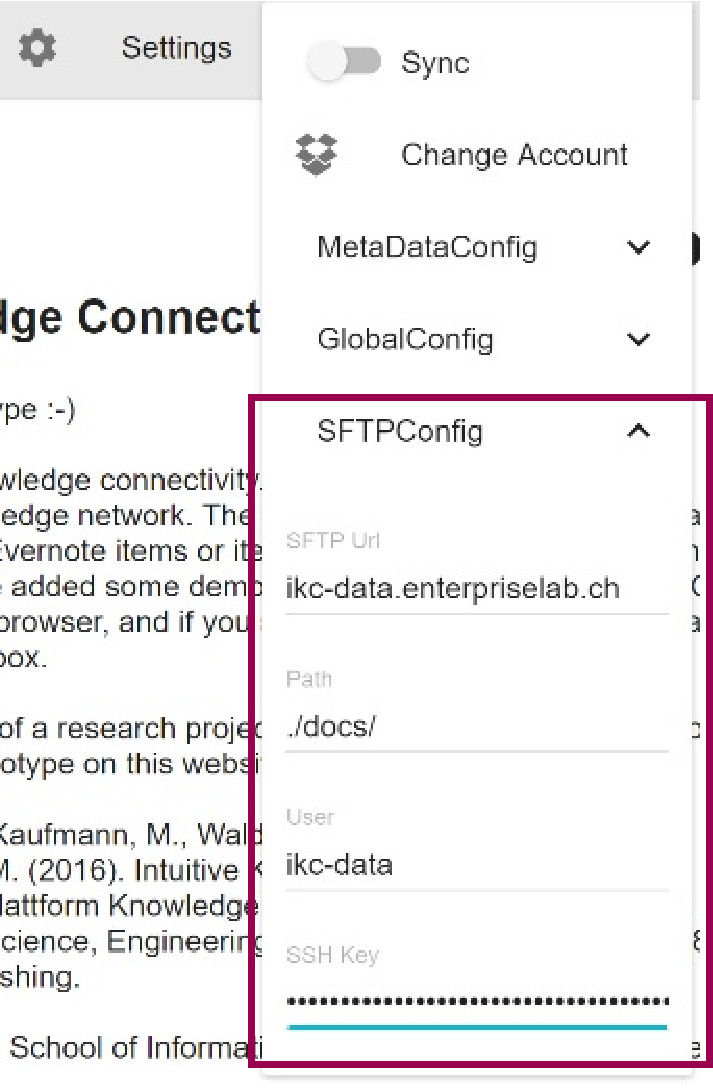
\includegraphics[width=1\linewidth]{Settings-SFTP}
    \caption{Datenquelle}
    \label{fig:sftp-config}
    \end{subfigure}
    \caption{Applikationskonfiguration}
\end{figure}
\end{landscape}
\newpage

\subsection{Keyphrase hinzufügen}
\autoref{fig:addtag} beschreibt den Vorgang, um einem Node eine \gls{Keyphrase} hinzuzufügen:
\begin{enumerate}
    \item Gewünschte \gls{Keyphrase} eingeben. 
    \item Mit der \textit{Tab}-Taste bestätigen.
\end{enumerate}

\begin{figure}[ht]
\centering
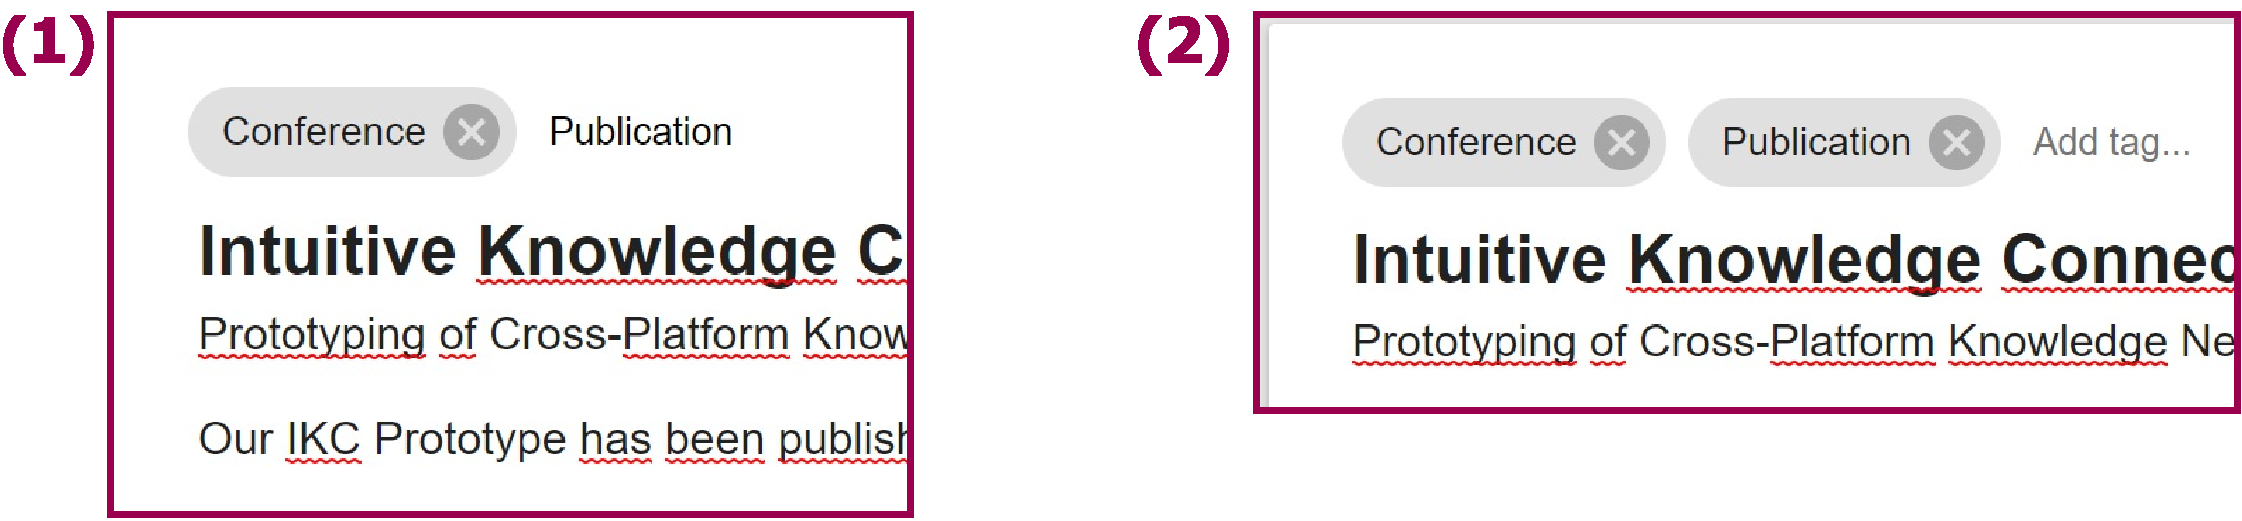
\includegraphics[width=1\textwidth]{AddTag}
\caption{Keyphrase hinzufügen}
\label{fig:addtag}
\end{figure}


\subsection{Keyphrase Vorschlag}
Beim Hinzufügen einer \gls{Keyphrase} werden Vorschläge gemacht. \autoref{fig:addtagautocomplete} beschreibt diesen Vorgang:
\begin{enumerate}
    \item Sobald eine Eingabe existiert, werden bestehende \gls{Keyphrase}[s] vorgeschlagen. Die Liste beschränkt sich jedoch auf bereits verwendete \gls{Keyphrase}[s].
    \item Nach der Auswahl der gewünschten \gls{Keyphrase} wird sie dem Node hinzugefügt.
\end{enumerate}
\begin{figure}[ht]
\centering
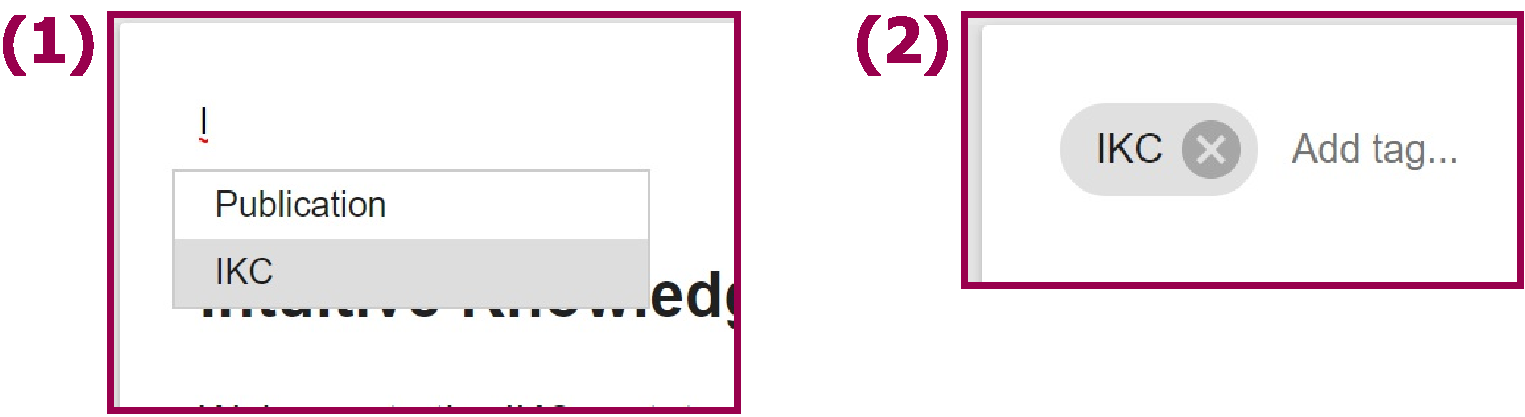
\includegraphics[width=1\textwidth]{TagAutocomplete}
\caption{Keyphrase Autovervollständigung}
\label{fig:addtagautocomplete}
\end{figure}


\subsection{Suche}
Die Suche innerhalb des Volltext-Index ist in die bereits bestehende Suche integriert. \autoref{fig:external-search} beschreibt diesen Vorgang:
\begin{enumerate}
    \item Der Suchbegriff kann in der Suchmaske eingegeben werden. Falls Ergebnisse innerhalb des \gls{ikc-core}[s] gefunden werden, erscheinen diese unmittelbar.
    \item Sobald die Suchanfrage abgearbeitet wurde, werden die Resultate dargestellt. Diese beinhalten, falls existent, auch externe Ergebnisse.
\end{enumerate}

\begin{figure}[ht]
\centering
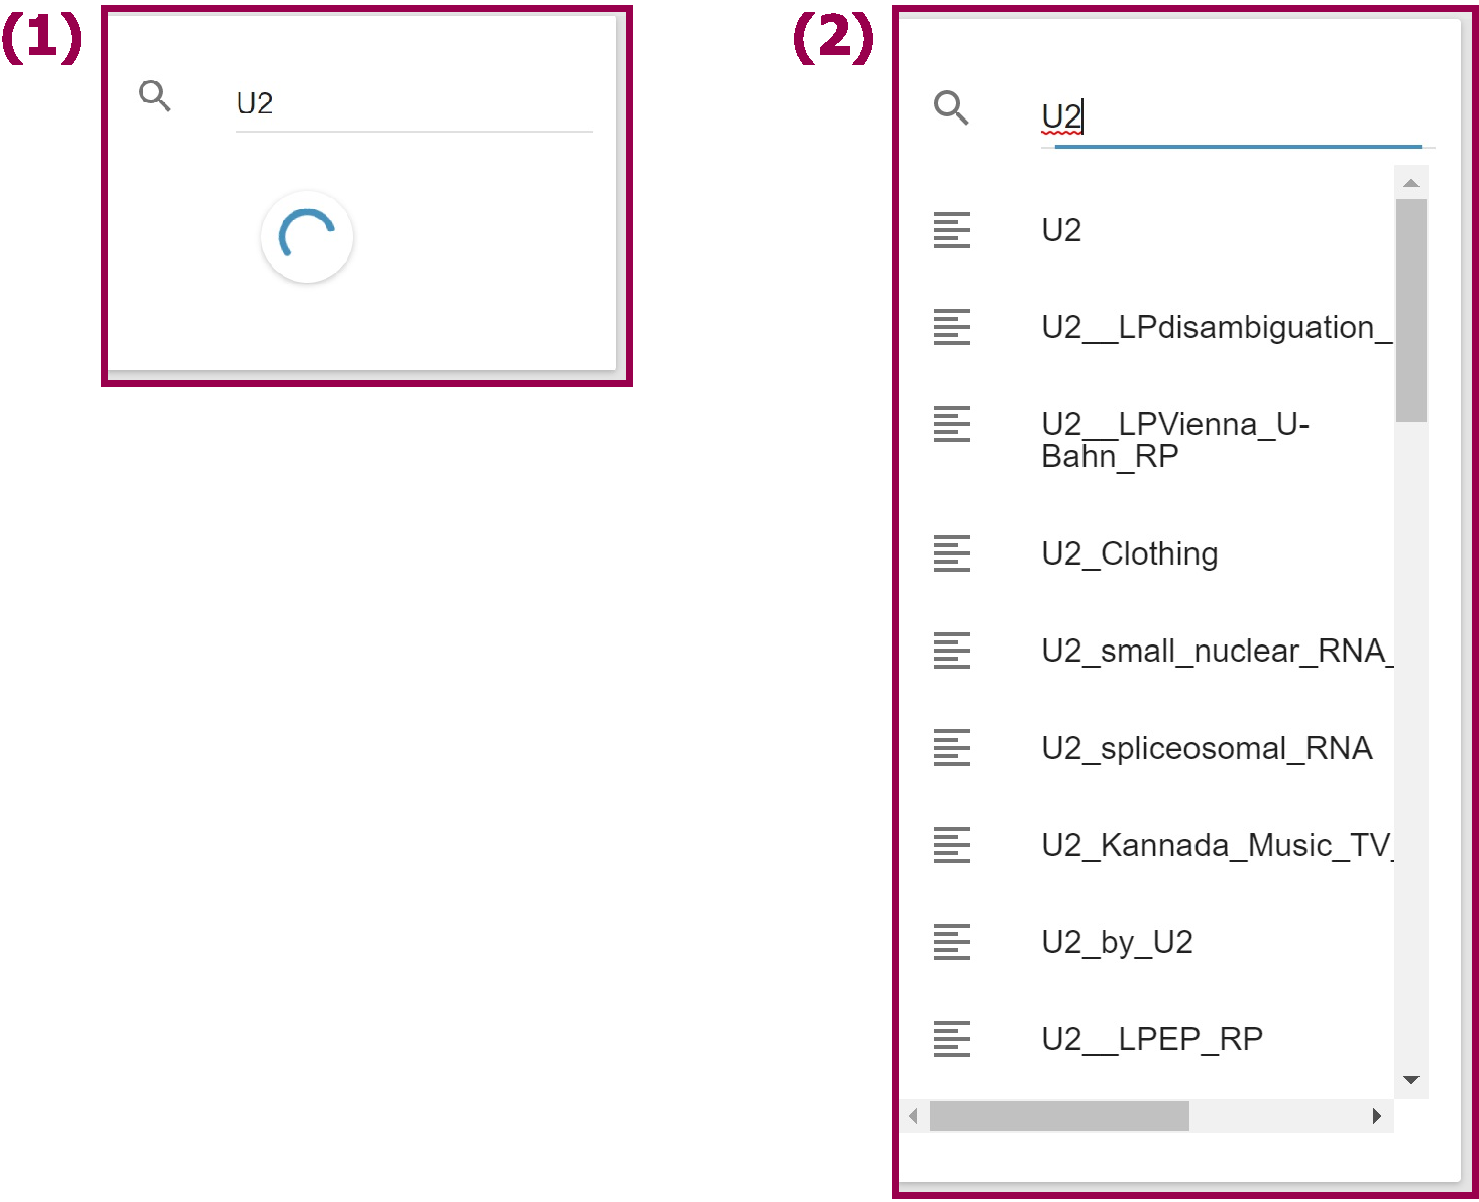
\includegraphics[width=1\textwidth]{Search}
\caption{Suche}
\label{fig:external-search}
\end{figure}

\subsection{Dokument auswählen}
\autoref{fig:select-doc} beschreibt, wie ein Dokument ausgewählt und angezeigt werden kann:
\begin{enumerate}
    \item Ein Dokument kann über die Suche oder durch einen Klick auf eine Verknüpfung ausgewählt werden: Beispiel: \textit{U2}.
    \item Zusammen mit dem Dokument werden relevante \gls{Keyphrase}[s] angezeigt.
\end{enumerate}

\begin{figure}[ht]
\centering
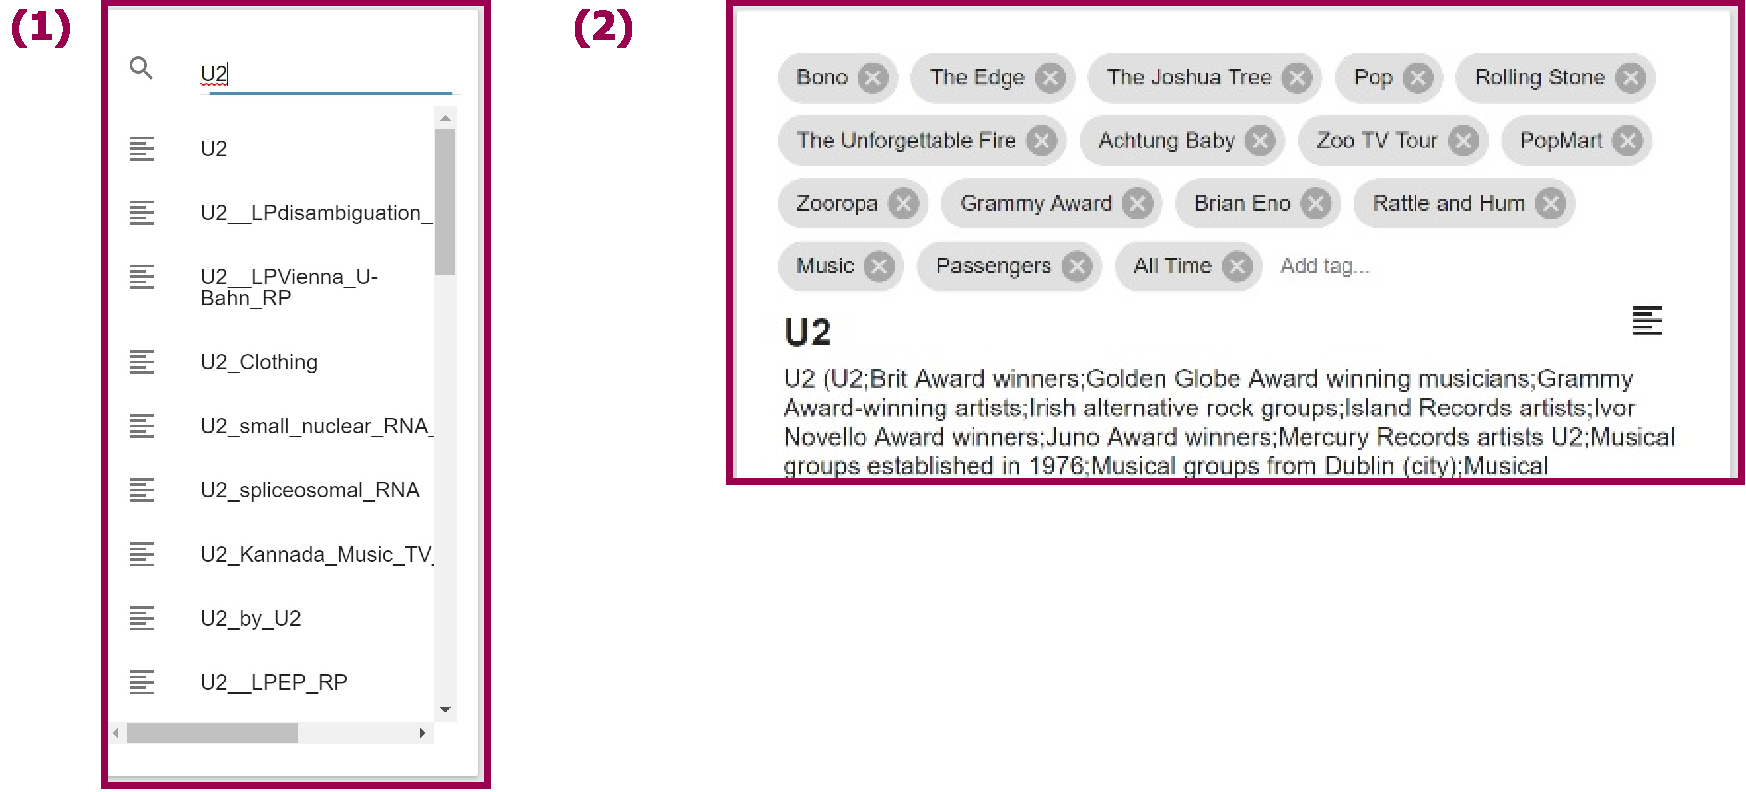
\includegraphics[width=1.2\textwidth]{SelectDocument}
\caption{Dokument auswählen}
\label{fig:select-doc}
\end{figure}

\subsection{Keyphrase auswählen}

Der Vorgang, der Anzeige einer \gls{Keyphrase} mit zugehörigen Dokumenten, wird \autoref{fig:select-keyphrase} aufgezeigt:
\begin{enumerate}
    \item Das entsprechende \gls{Keyphrase} auswählen. Beispiel: \textit{Bono}.
    \item Anschliessend wird die \gls{Keyphrase} als Node dargestellt und mit allen Dokumenten verlinkt, welche diese enthalten. 
\end{enumerate}

\begin{figure}[ht]
\centering
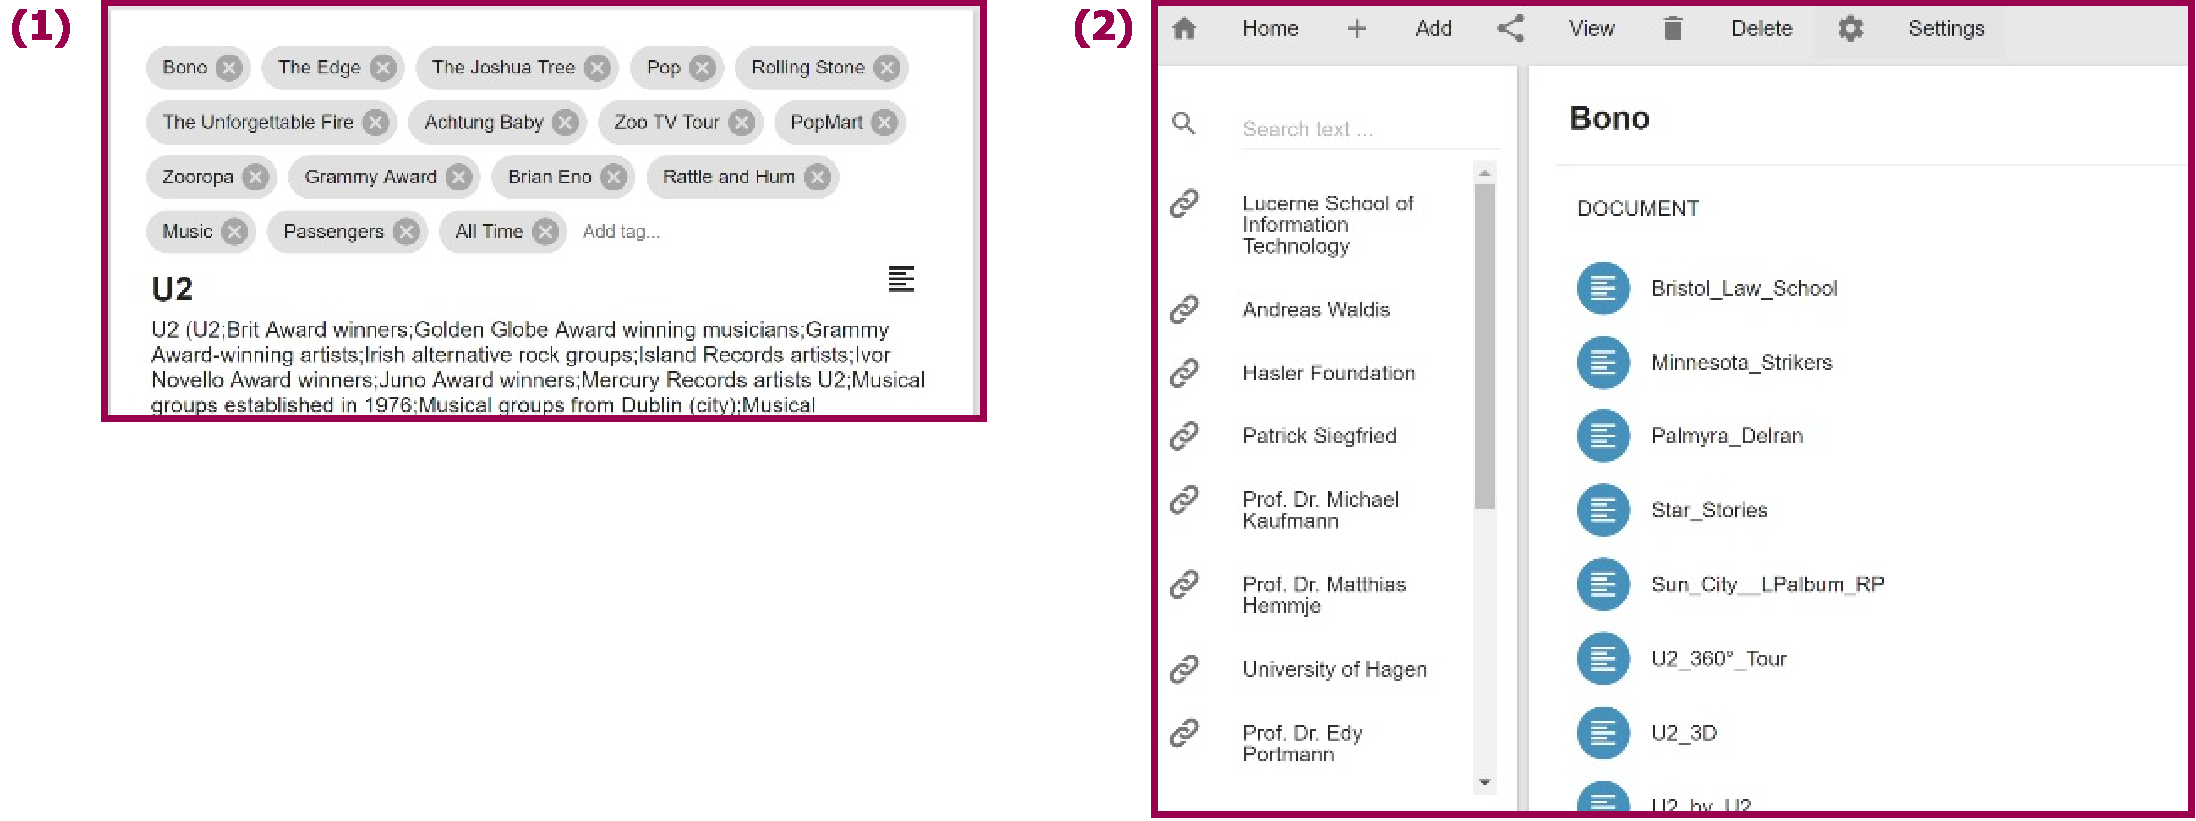
\includegraphics[width=1.2\textwidth]{SelectKeyphrase}
\caption{Keyphrase auswählen}
\label{fig:select-keyphrase}
\end{figure}

\subsection{Keyphrase abfragen}
\gls{Keyphrase}[s] können auch über die Suche abgefragt werden. \autoref{fig:query-keyphrase} zeigt diesen Vorgang:
\begin{enumerate}
    \item Die gewünschte \gls{Keyphrase} eingeben und auswählen. Beispiel: \textit{Bono}
    \item Nun wird es zusammen mit den Dokumenten, welche es enthalten dargestellt.
\end{enumerate}

\begin{figure}[ht]
\centering
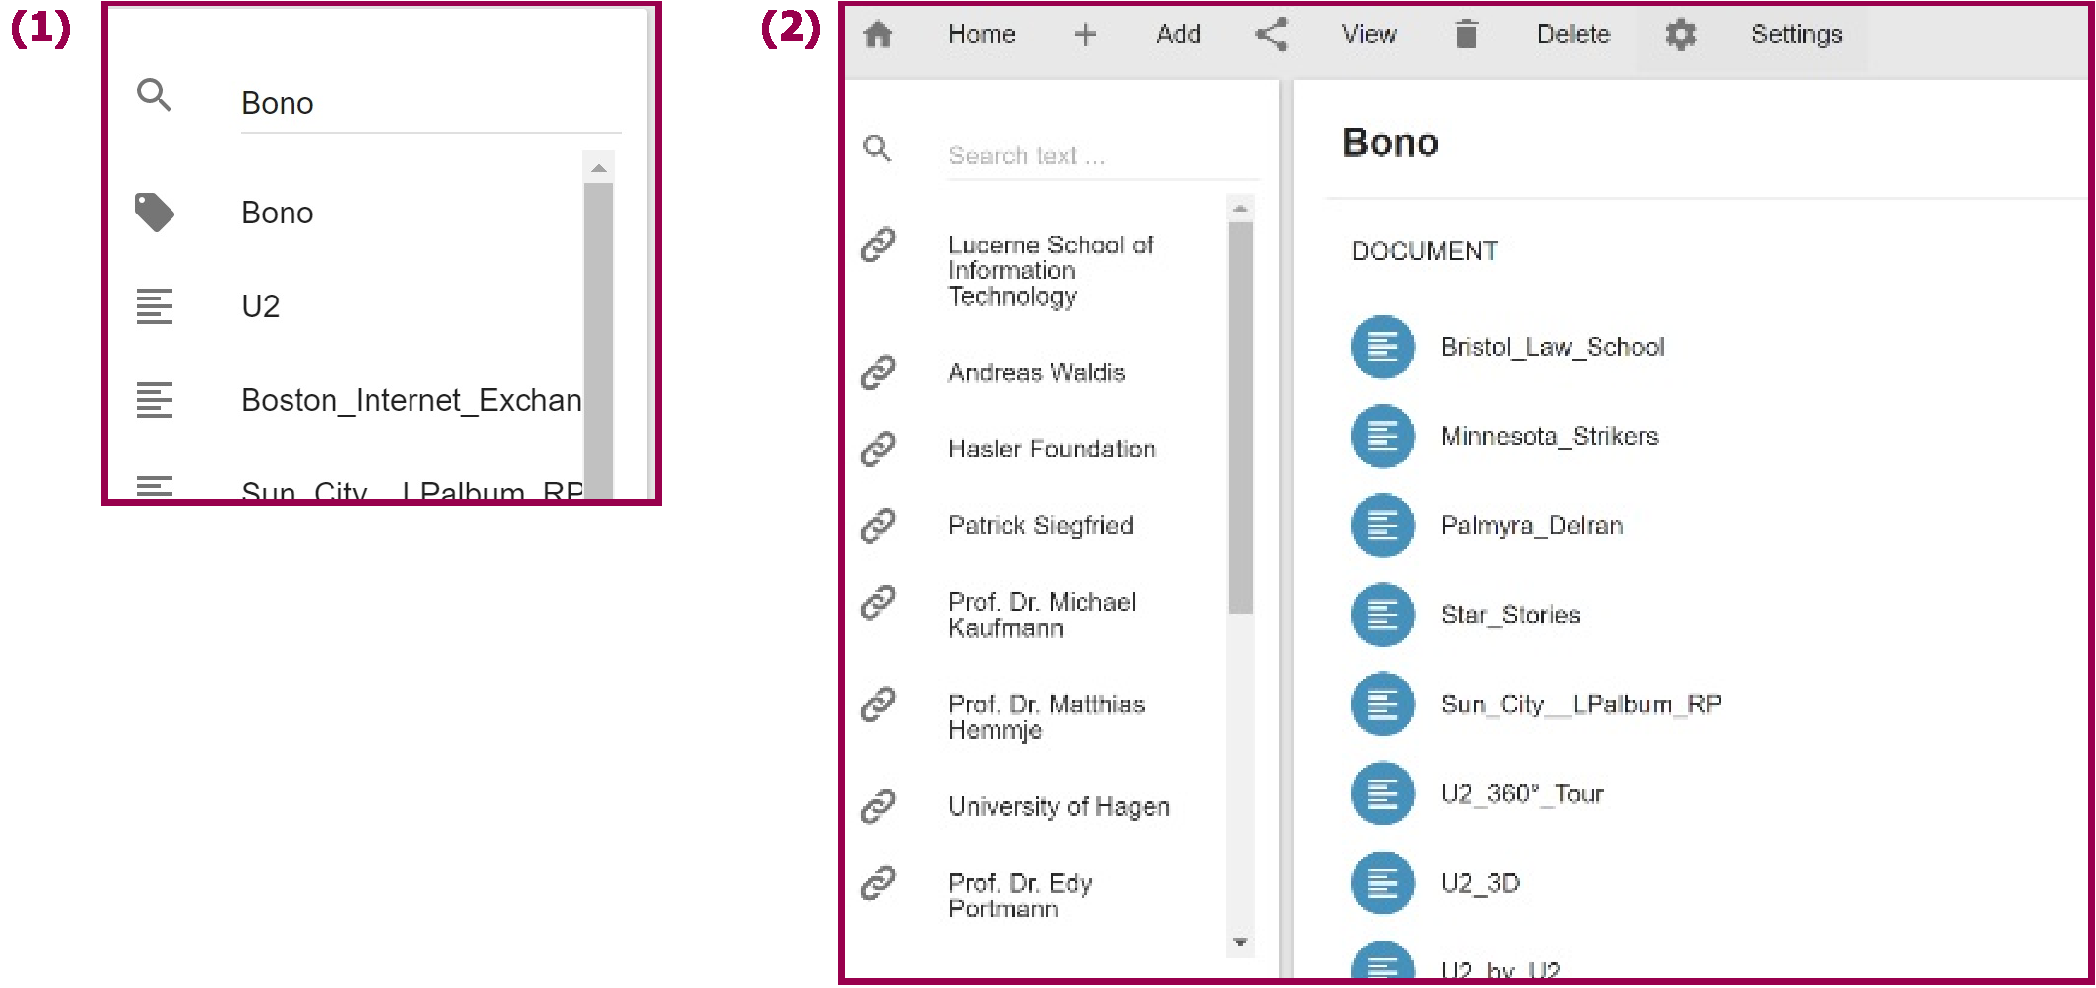
\includegraphics[width=1.2\textwidth]{QueryKeyphrase}
\caption{Keyphrase auswählen}
\label{fig:query-keyphrase}
\end{figure}


